Este apêndice reúne as telas do osciloscópio dos ensaios em bancada (Seção~\ref{sec:bancada}), feitos com um Tektronix TBS1102B em modo de amostragem simples e acoplamento AC. O relógio do osciloscópio estava adiantado em um dia: as telas indicam 6 de outubro de 2026, mas as medidas foram feitas em 5 de outubro. Para cada tela, o repositório guarda, na pasta \cod{analog/resultados/}, a imagem, os pontos do canal em \ac{csv} e a configuração do osciloscópio.

\section{Saída da placa}

As telas a seguir foram medidas na saída do seguidor de tensão (U1D), onde antes ficava o estágio classe AB. Nas medidas no domínio do tempo, o contador do canto inferior direito indica a frequência do sinal; na forma arbitrária, a tabela do \acs{ecg} tem dois batimentos por período, e o contador mede o dobro da frequência pedida.

\begin{figure}
	\caption{Saída da placa: seno de 10~Hz (100~mV/div e 25~ms/div).}
	\label{fig:osc_ab_seno_10Hz}
	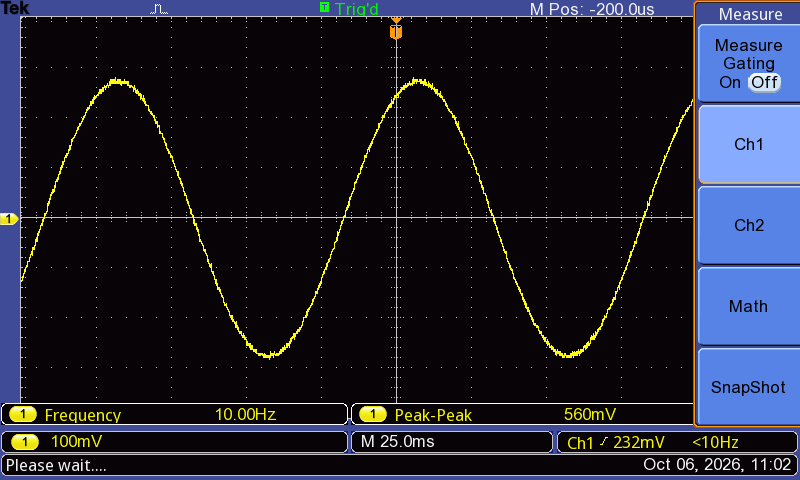
\includegraphics[width=0.8\textwidth]{./figuras/osc_ab_seno_10Hz}
	\legend{Fonte~---~Autoria própria.}
\end{figure}

\begin{figure}
	\caption{Saída da placa: seno de 100~Hz (100~mV/div e 2,5~ms/div).}
	\label{fig:osc_ab_seno_100Hz}
	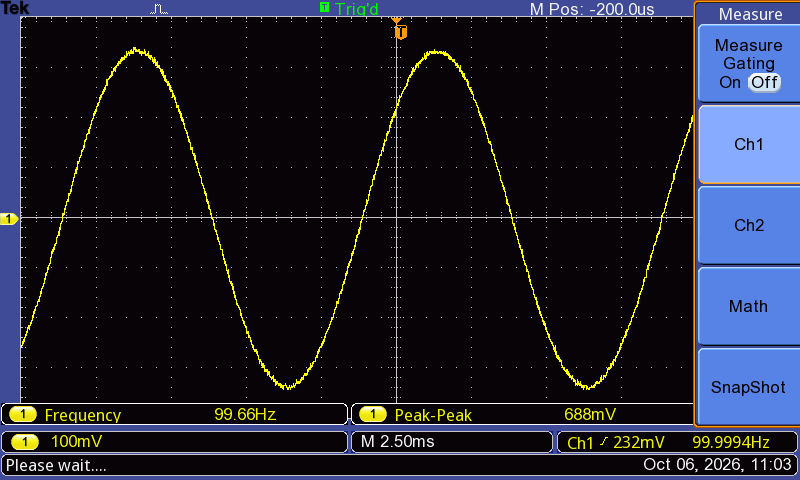
\includegraphics[width=0.8\textwidth]{./figuras/osc_ab_seno_100Hz}
	\legend{Fonte~---~Autoria própria.}
\end{figure}

\begin{figure}
	\caption{Saída da placa: seno de 1~kHz (100~mV/div e 500~\(\mu\)s/div).}
	\label{fig:osc_ab_seno_1kHz}
	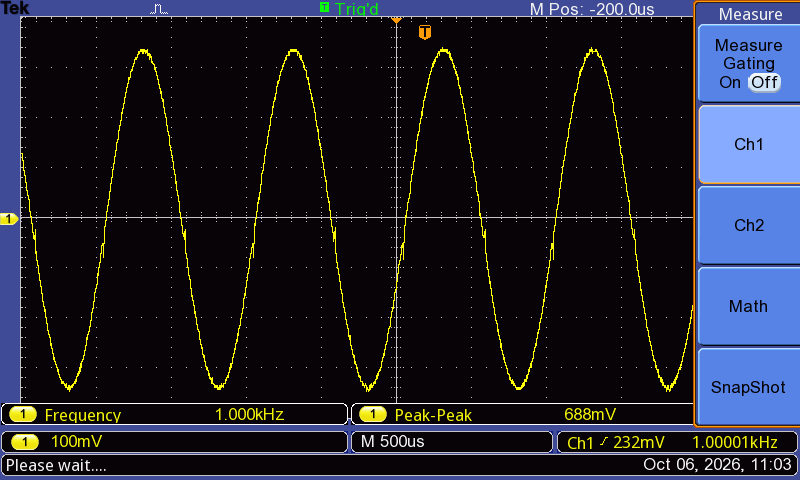
\includegraphics[width=0.8\textwidth]{./figuras/osc_ab_seno_1kHz}
	\legend{Fonte~---~Autoria própria.}
\end{figure}

\begin{figure}
	\caption{Saída da placa: seno de 10~kHz (100~mV/div e 50~\(\mu\)s/div).}
	\label{fig:osc_ab_seno_10kHz}
	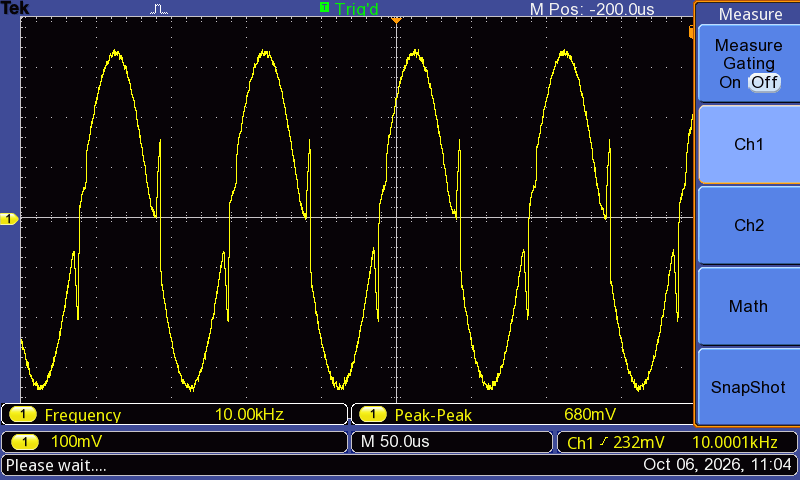
\includegraphics[width=0.8\textwidth]{./figuras/osc_ab_seno_10kHz}
	\legend{Fonte~---~Autoria própria.}
\end{figure}

\begin{figure}
	\caption{Saída da placa: rampa de 100~Hz (100~mV/div e 2,5~ms/div).}
	\label{fig:osc_ab_rampa_100Hz}
	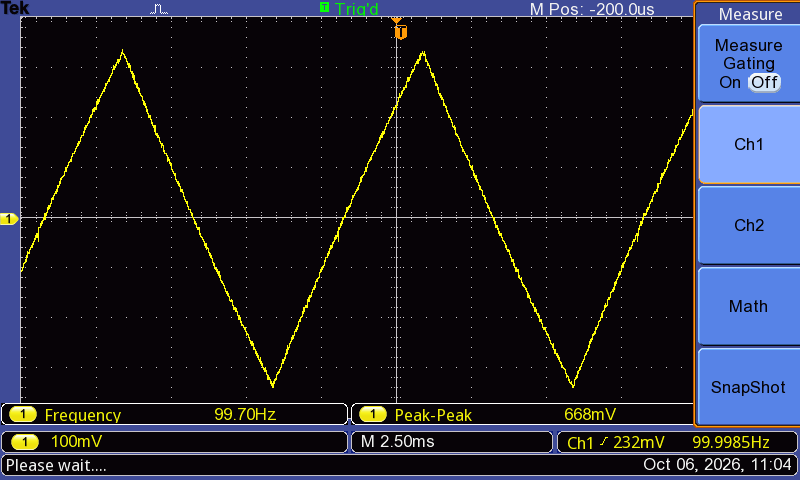
\includegraphics[width=0.8\textwidth]{./figuras/osc_ab_rampa_100Hz}
	\legend{Fonte~---~Autoria própria.}
\end{figure}

\begin{figure}
	\caption{Saída da placa: função sinc de 100~Hz (100~mV/div e 2,5~ms/div).}
	\label{fig:osc_ab_sinc_100Hz}
	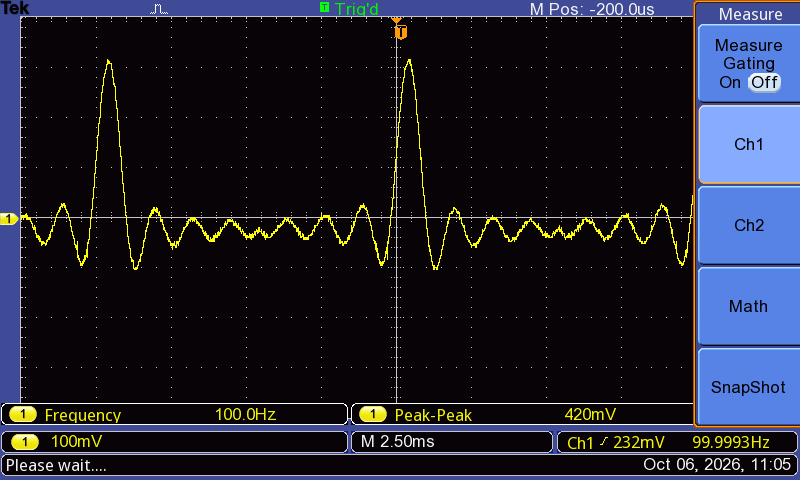
\includegraphics[width=0.8\textwidth]{./figuras/osc_ab_sinc_100Hz}
	\legend{Fonte~---~Autoria própria.}
\end{figure}

\begin{figure}
	\caption{Saída da placa: forma arbitrária com a tabela do \acs{ecg}, em 100~Hz (100~mV/div e 2,5~ms/div).}
	\label{fig:osc_ab_ecg_100Hz}
	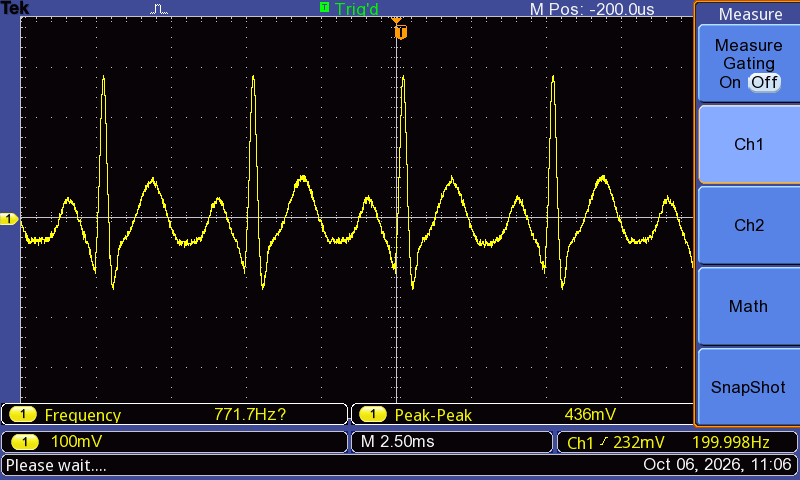
\includegraphics[width=0.8\textwidth]{./figuras/osc_ab_ecg_100Hz}
	\legend{Fonte~---~Autoria própria.}
\end{figure}

\begin{figure}
	\caption{Saída da placa: espectro do seno de 100~Hz, até 2,5~kHz (10~dB/div e 250~Hz/div, amostragem de 5~kS/s).}
	\label{fig:osc_ab_fft_pico_harmonico}
	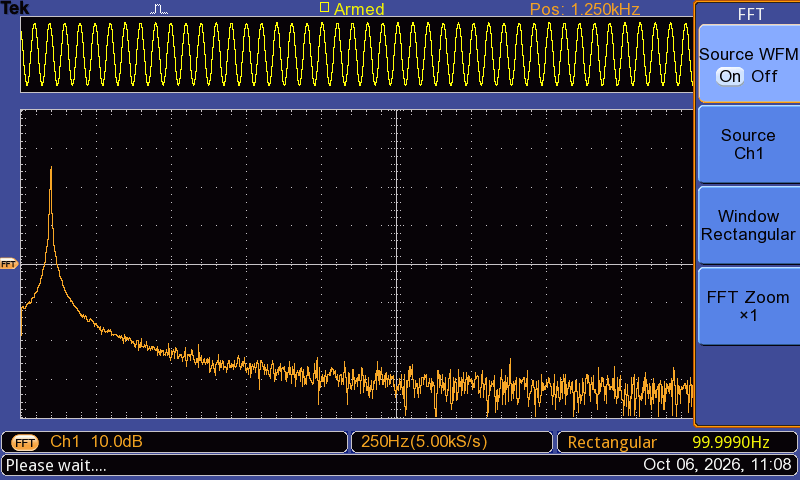
\includegraphics[width=0.8\textwidth]{./figuras/osc_ab_fft_pico_harmonico}
	\legend{Fonte~---~Autoria própria.}
\end{figure}

\begin{figure}
	\caption{Saída da placa: espectro do seno de 100~Hz, até 50~MHz (10~dB/div e 5~MHz/div, amostragem de 100~MS/s).}
	\label{fig:osc_ab_fft_aliasing}
	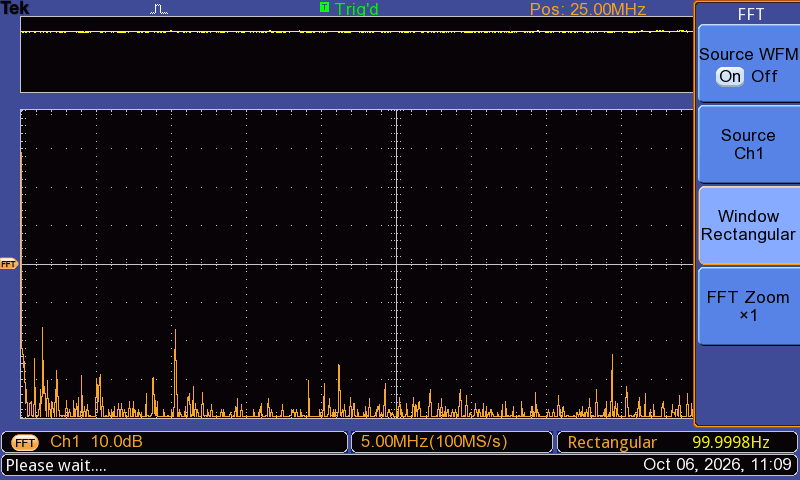
\includegraphics[width=0.8\textwidth]{./figuras/osc_ab_fft_aliasing}
	\legend{Fonte~---~Autoria própria.}
\end{figure}

\begin{figure}
	\caption{Saída da placa: espectro do seno de 10~kHz amostrado abaixo da taxa de Nyquist (10~dB/div e 125~Hz/div, amostragem de 2,5~kS/s).}
	\label{fig:osc_ab_fft_10kHz_subamostrado}
	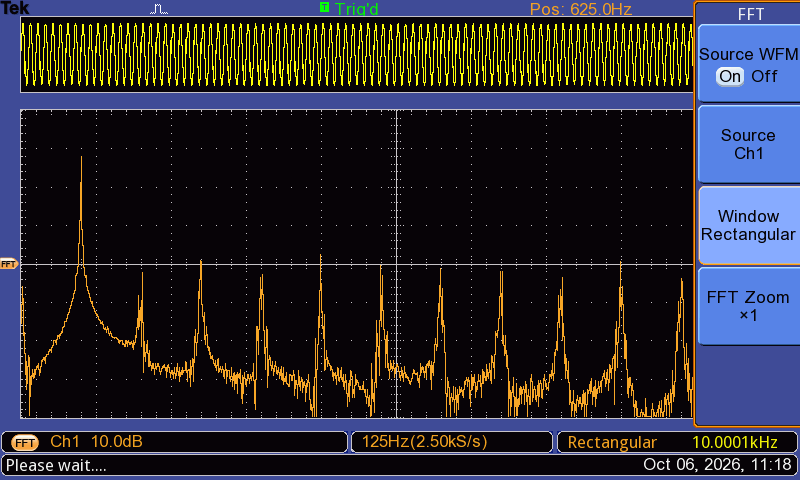
\includegraphics[width=0.8\textwidth]{./figuras/osc_ab_fft_10kHz_subamostrado}
	\legend{Fonte~---~Autoria própria.}
\end{figure}

\clearpage
\section{Saída do subtrator}

As telas a seguir foram medidas na saída do amplificador de diferenças (U1A), logo após o \acs{dac}.

\begin{figure}
	\caption{Saída do subtrator: seno de 10~kHz (500~mV/div e 50~\(\mu\)s/div).}
	\label{fig:osc_subtrator_seno_10kHz}
	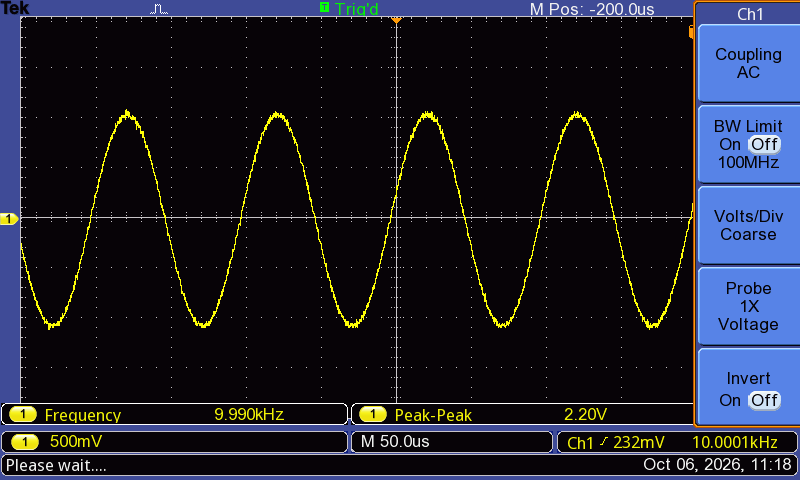
\includegraphics[width=0.8\textwidth]{./figuras/osc_subtrator_seno_10kHz}
	\legend{Fonte~---~Autoria própria.}
\end{figure}

\begin{figure}
	\caption{Saída do subtrator: seno de 20~kHz (500~mV/div e 25~\(\mu\)s/div).}
	\label{fig:osc_subtrator_seno_20kHz}
	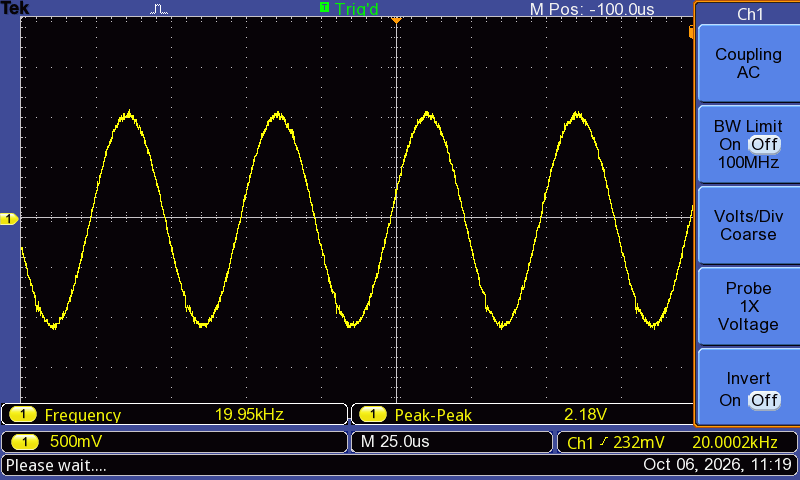
\includegraphics[width=0.8\textwidth]{./figuras/osc_subtrator_seno_20kHz}
	\legend{Fonte~---~Autoria própria.}
\end{figure}

\begin{figure}
	\caption{Saída do subtrator: seno de 30~kHz (500~mV/div e 25~\(\mu\)s/div).}
	\label{fig:osc_subtrator_seno_30kHz}
	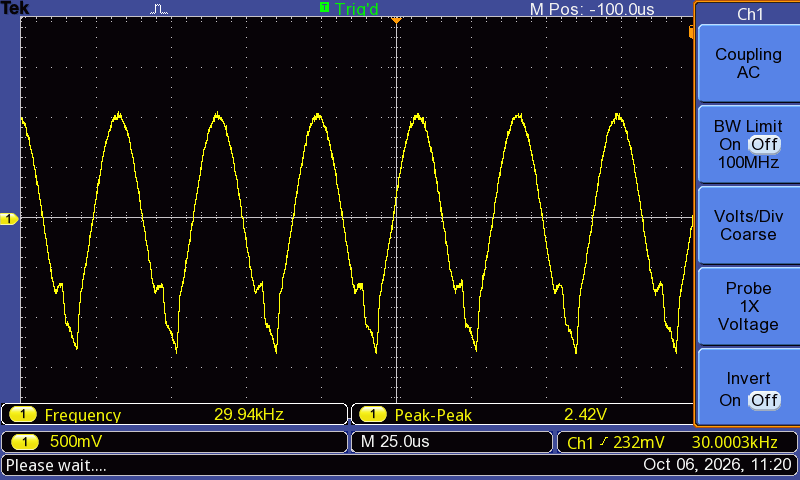
\includegraphics[width=0.8\textwidth]{./figuras/osc_subtrator_seno_30kHz}
	\legend{Fonte~---~Autoria própria.}
\end{figure}
